% TODO [E]: Cela part sur les chapeaux de roues, ensuite on a l'impression qu'il
% n'y a que l'IA comme analyse statique et un peu le typage

Dans ce chapitre, nous présentons un tour d'horizon des techniques existantes
permettant d'analyser des programmes. Un accent est mis sur la propriété de
sécurité décrite dans le chapitre~\ref{cha:os}, mais on ne se limite pas à
celle-ci.

L'analyse statique de programmes est un sujet de recherche actif depuis
l'apparition de la science informatique. On commence par en présenter une
classification, puis on montrera des exemples pertinents permettant d'analyser
du code système ou embarqué.

\section{Taxonomie}

\paragraph{Techniques statiques et dynamiques}

L'analyse peut être faite au moment de la compilation, ou au moment de
l'exécution. En général on peut obtenir des informations plus précises de
manière dynamique, mais cela ne prend en compte que les parties du programme qui
seront vraiment exécutées. Un autre problème des techniques dynamiques est qu'il
est souvent nécessaire d'instrumenter l'environnement d'exécution (ce qui ---
dans le cas où cela est possible --- peut se traduire par un impact en
performances). L'approche statique, en revanche, nécessite de construire à
l'arrêt une carte mentale du programme, ce qui n'est pas toujours possible dans
certains langages.

Pour s'assurer de la correction d'un programme, on ne peut pas s'appuyer
uniquement sur des tests --- ou de manière générale sur des analyses dynamiques
--- car même avec des tests exhaustifs, il est impossible d'étudier l'ensemble
complet de tous les comportements possibles. Par exemple, si un bug se présente
lors d'une interaction entre deux composants qui n'a pas été testée, il passera
inaperçu. Pour cette raison, la plupart des analyses présentées ici sont
statiques.

\paragraph{Cohérence et complétude}

Le but d'une analyse statique est de catégoriser les programmes selon s'ils
satisfont ou non un ensemble de propriétés fixées à l'avance. Malheureusement,
ceci n'est pas possible : l'ensemble des valeurs possibles lors de l'exécution
d'un programme n'est pas un ensemble calculable (théorème de Rice~\cite{rice}).
Autrement dit, il ne peut exister une procédure de décision prenant un programme
et le déclarant correct ou incorrect.

Il n'est donc pas possible d'écrire un analyseur statique parfait, ne se
trompant jamais. Toute technique statique va donc de se retrouver dans au moins
un des cas suivants :

\begin{itemize}
\item
  un programme valide (pour une propriété donnée) est rejeté : on parle de
  \emph{faux positif}.
\item
  un programme invalide n'est pas détecté : on parle de
  \emph{faux négatif}.
\end{itemize}

En général on préfère s'assurer que les programmes acceptés possèdent la
propriété recherchée, quitte à en rejeter certains.

Par ailleurs la plupart des techniques ne concernent que les programmes qui
terminent. On étudie donc la correction, ou les propriétés des termes
convergents. Prouver automatiquement que l'exécution ne boucle pas est une
propriété toute autre qui n'est pas ici considérée.

\section{Méthodes syntaxiques}

L'analyse la plus simple consiste à traiter un programme comme du texte, et à y
rechercher des motifs dangereux. Ainsi, utiliser des outils comme \texttt{grep}
permet parfois de trouver un grand nombre de vulnérabilités~\cite{SpenderGrep}.

On peut continuer cette approche en recherchant des motifs mais en étant
sensible à la syntaxe et au flot de contrôle du programme. Cette notion de
\emph{semantic grep} est présente dans l'outil Coccinelle
\cite{coccinelle09,coccinelle11} : on peut définir des
\emph{patches sémantiques} pour détecter ou modifier des constructions
particulières.

%TODO lire coccinelle09

\section{Interprétation abstraite}

L'interprétation abstraite est une technique d'analyse générique qui permet de
simuler statiquement tous les comportements d'un programme Cousot
\cite{Cousot77,Cousot92-1}. Un exemple d'application est de calculer les bornes
de variations des variables pour s'assurer qu'aucun débordement de tableau n'est
possible~\cite{AllamigeonHymansSSTIC07}.

L'idée est d'associer à chaque ensemble concret des valeurs, une représentation
abstraite. Sur celle-ci, on peut définir des opérations indépendantes de la
valeur exacte des données, mais préservant l'abstraction. Par exemple, les
règles comme $"-" × "-" = "+"$ définissent le domaine abstrait des signes. Les
domaines ont une structure de treillis, c'est-à-dire qu'ils possèdent les
notions d'ordre partiel et d'union de valeurs (figure~\ref{fig:dom-sig}). En
calculant les valeurs extremales d'une variable, on obtient le domaine des
intervalles.

\begin{figure}%{{{
\centering

\begin{minipage}{0.4\textwidth}
  \begin{tikzpicture}
  \node at (1, 2) (t) {$\top$};
  \node at (0, 1) (m) {$-$};
  \node at (1, 1) (z) {$0$};
  \node at (2, 1) (p) {$+$};
  \node at (1, 0) (b) {$\bot$};
  \draw (t) -- (p) -- (b);
  \draw (t) -- (m) -- (b);
  \draw (t) -- (z) -- (b);
  \end{tikzpicture}
\end{minipage}
\begin{minipage}{0.4\textwidth}
  \begin{align*}
  γ~(-) = & ℝ^- \\
  γ~(0) = & \{0\} \\
  γ~(+) = & ℝ^+ \\
  \end{align*}
\end{minipage}

\caption{Domaine des signes}
\label{fig:dom-sig}
\end{figure}%}}}

Ces domaines ne capturent aucune relation entre variables. ils sont dits non
relationnels. Lorsque plusieurs variables sont analysées en même temps, utiliser
de tels domaines consiste à considérer un produit cartésien d'ensembles
abstraits (figure~\ref{fig:dom-cartesien}).

Des domaines abstraits plus précis permettent de retenir celles-ci. Pour ce
faire, il faut modéliser l'ensemble des valeurs des variables comme un tout.
Parmi les domaines relationnels courants on peut citer : le domaine des
polyèdres, permet de retenir tous les invariants affines entre fonctions
(figure~\ref{fig:dom-poly}) ; le domaine des zones, permettant de représenter
des relations affines de la forme $v_i - v_j \le c$ (figure~\ref{fig:dom-zones})
; ou encore le domaine des octogones qui est un compromis entre les polyèdres et
les zones. Il permet de représenter les relations $\pm v_i \pm v_j \le c$
(figure~\ref{fig:dom-octo}).

\begin{figure}%{{{

  \centering

  %{{{
  \subbottom[Domaine non relationnel]{
    \label{fig:dom-cartesien}
      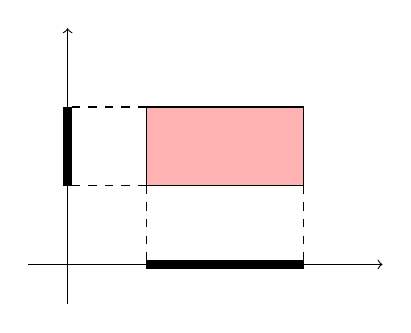
\begin{tikzpicture}
      \draw[->] (0,-0.5) -- (0,3);
      \draw[->] (-0.5,0) -- (4,0);
%
      \draw[fill=red!30] (1,1) rectangle (3,2);
%
      \draw[dashed] (3,1) -- (3,0);
      \draw[dashed] (1,1) -- (1,0);
%
      \draw[dashed] (1,2) -- (0,2);
      \draw[dashed] (1,1) -- (0,1);
%
      \draw[line width=3pt] (0,1) -- (0,2);
      \draw[line width=3pt] (3,0) -- (1,0);
%
      \end{tikzpicture}
  }%}}}
  \subbottom[Domaine des polyèdres]{%{{{
    \label{fig:dom-poly}
%
    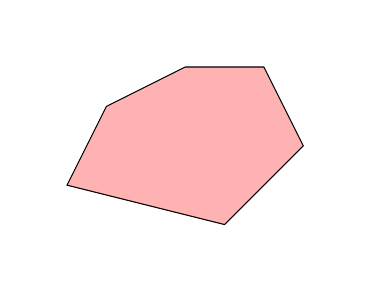
\begin{tikzpicture}[scale=0.5]
    \path[use as bounding box] (0,0) rectangle (8, 6);
%
    \draw[fill=red!30] (1,2) -- (2,4) -- (4,5) -- (6,5) -- (7,3) -- (5,1) -- cycle;
%
    \end{tikzpicture}
  }%}}}

  \subbottom[Domaine des zones]{%{{{
    \label{fig:dom-zones}
%
    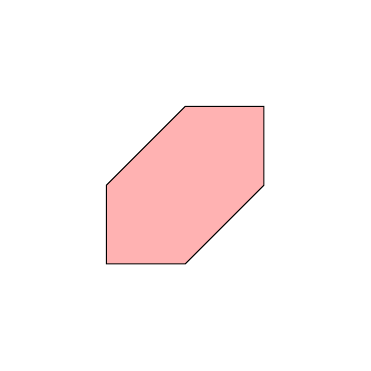
\begin{tikzpicture}
    \path[use as bounding box] (0,0) rectangle (4,4);
%
    \draw[fill=red!30] (1,2) -- (2,3) -- (3,3) -- (3,2) -- (2,1) -- (1,1) -- cycle;
%
    \end{tikzpicture}
  }%}}}
  \subbottom[Domaine des octaèdres]{%{{{
    \label{fig:dom-octo}
%
    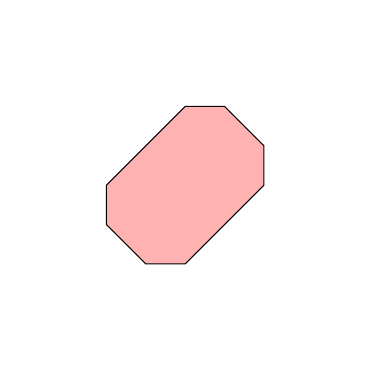
\begin{tikzpicture}
    \path[use as bounding box] (0,0) rectangle (4,4);
%
    \draw[fill=red!30] (1,1.5) -- (1,2) -- (2,3) -- (2.5,3) -- (3,2.5) -- (3,2) -- (2,1) -- (1.5,1) -- cycle;
%
    \end{tikzpicture}
  }%}}}

  \caption{Quelques domaines abstraits}
  \label{fig:dom-abstraits}
\end{figure}%}}}

En plus des domaines numériques, il est nécessaire d'employer des domaines
spécialisés dans la modélisation de la mémoire. Cela est nécessaire pour pouvoir
"suivre" les pointeurs. Par exemple, on peut représenter un pointeur par un
ensemble de variables possiblement pointées et une valeur abstraite représentant
le décalage (\emph{offset}) du pointeur par rapport au début de la zone mémoire.
Cette valeur peut elle-même être abstraite par un domaine numérique.

Au delà des domaines eux-mêmes, l'analyse se fait sous forme d'un calcul de
point fixe. La manière la plus simple est d'utiliser un algorithme de
\emph{liste de travail}, décrit par exemple dans~\cite{tapsoft95}. Les
raffinement en revanche sont nombreux.

Dès~\cite{Cousot77} il est remarqué que la terminaison de l'analyse n'est
assurée que si le treillis des valeurs abstraites est de hauteur finie, ou qu'un
opérateur d'élargissement (\emph{widening}) $\nabla$ est employé. L'idée est
qu'une fois qu'on a calculé quelques termes d'une suite croissante, on peut
réaliser une projection de celle ci. Par exemple, dans le domaine des
intervalles, $[0;2]~\nabla~[0;3] = [0;+\infty[$. On atteint alors un point fixe
mais qui est plus grand que celui qu'on aurait obtenu sans cette accélération :
on perd en précision. Pour en gagner, on peut redescendre sur le treillis des
points fixe avec une suite d'itérations décroissantes \cite{granger}. Dans
l'itération de point fixe, il est possible d'obtenir les résultats de manière
plus efficace en choisissant un ordre particulier dans les calculs des
sous-itérations\cite{policy}.

En termes d'ingéniérie logicielle, implanter un analyseur statique est un défi
en soi. En plus des domaines abstraits, d'un itérateur, il faut traduire le code
source à analyser dans un langage, et traduire les résultats de l'analyse en un
ensemble d'"alarmes" à présenter à l'utilisateur.

Pour des retours d'expérience plus détaillés, on peut se référer aux descriptions d'
Astrée~\cite{Astree04,Astree05,AstreeScale},
CGS~\cite{cgs},
ou Coverity~\cite{coverityBillion}.

Cette technique est très puissante mais possède plusieurs inconvénients. D'une
part, pour réaliser une analyse interprocédurale il faut partir d'un point en
particulier du programme (comme la fonction \texttt{main}). Cette hypothèse
n'est pas facilement satisfaite dans un noyau de système d'exploitation, qui
possède de nombreux points d'entrée. D'autre part, elle remonte de nombreuses
fausses alarmes, puisqu'elle nécessite d'avoir une vue précise du programme.

\section{Typage}

\paragraph{Systèmes ad hoc}

Les systèmes de types les plus simples expriment des contrats esssentiellement
liés à la sûreté d'exécution, pour ne pas utiliser des valeurs de types
incompatibles entre eux. Mais il est possible d'étendre le langage avec des
annotations plus riches : par exemple en vérifiant statiquement que des listes
ne sont pas vides\cite{lightweight-static-capabilities}, ou dans le domaine de
la sécurité, d'empêcher des fuites d'information~\cite{LZ06a}.

\paragraph{Qualificateurs de types}

Dans le cas particulier des vulnérabilités liées à une mauvaise utilisation de
la mémoire, les développeurs du noyau Linux ont ajouté un système d'annotations
au code source. Un pointeur peut être décoré d'une annotation
\texttt{\_\_kernel} ou \texttt{\_\_user} selon s'il est sûr ou pas. Celle-ci
sont ignorées par le compilateur, mais un outil d'analyse statique ad-hoc nommé
Sparse~\link{sparse}~\cite{TorvaldsSparse} % TODO citer un seul peut être
utilisé pour détecter les cas les plus simples d'erreurs. Il demande aussi au
programmeur d'ajouter beaucoup d'annotations dans le programme. % TODO
quantifier

Ce système d'annotations sur les types a été formalisé sous le nom de
\emph{qualificateurs de types}~\cite{toplas-quals} : chaque type peut être
décoré d'un ensemble de qualificateurs (à la manière de \texttt{const}), et des
règles de typage permettent d'établir des propriétés sur le programme.

Plus précisément, les jugements de typage de la forme $Γ ⊢ e : t$ sont remplacés
par des jugements de typage qualifiés $Γ ⊢ e : t~q$. Les qualificateurs $q$
permettent d'exprimer plusieurs jugements.
Par exemple, pointeurs on peut étudier le fait qu'une variable soit constante ou
pas, que sa valeur soit connue à la compilation, ou encore qu'elle puisse être
nulle ou pas.
La
spécificité de ce système est que les qualificateurs sont ordonnés, du plus
spécifique au moins spécifique, et que l'on forme alors un treillis à partir de
ces informations. Partant des deux caractéristiques précédentes, on forme le
treillis de la figure~\ref{fig:cqual-treillis}.

\begin{figure}
\centering
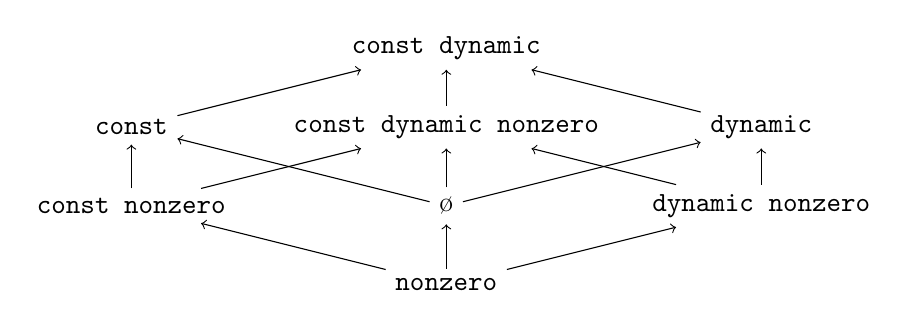
\begin{tikzpicture}

\node             (A) {\texttt{const dynamic}};
\node[below of=A] (C) {\texttt{const dynamic nonzero}};
\node[left of=C, node distance=4cm]  (B) {\texttt{const}};
\node[right of=C, node distance=4cm] (D) {\texttt{dynamic}};
\node[below of=B] (E) {\texttt{const nonzero}};
\node[below of=C] (F) {ø};
\node[below of=D] (G) {\texttt{dynamic nonzero}};
\node[below of=F] (H) {\texttt{nonzero}};

\foreach \s/\d in {H/E,H/F,H/G,E/B,E/C,F/B,F/C,F/D,G/C,G/D,B/A,C/A,D/A}
  \draw[->] (\s) -- (\d);

\end{tikzpicture}

\caption{Treillis de qualificateurs}
\label{fig:cqual-treillis}
\end{figure}

Cette relation d'ordre $\preceq$ entre qualificateurs, induit une relation de
sous-typage $\sqsubseteq$ entre les types qualifiés : si $q \preceq q'$, alors
$t~q \sqsubseteq t~q'$.

Ces analyses ont été implantée dans l'outil CQual. Ce système peut servir à
inférer les annotations \texttt{const}~\cite{pldi99}, à l'analyse de souillure
pour les chaînes de format~\cite{usenix01} (pouvant poser des problèmes de
sécurité~\cite{format-string-attacks}) et des propriétés dépendantes du flot de
contrôle, comme des invariants sur les verrous~\cite{pldi02}, à rapprocher du
concept de \emph{typestates}~\cite{tse12-typestate}. Il a également été appliqué
à la classe de vulnérabilités sur les pointeurs utilisateurs dont il est ici
l'objet~\cite{cquk-usenix04}.

\section{Analyse de code système}

Les logiciels système demandant des garanties de sécurité et de fiabilité, de
nombreuses analyses \emph{ad-hoc} ciblent les noyaux de systèmes d'exploitation.

Ajouter un système de types forts à C est l'idée centrale de
CCured~\cite{ccured-toplas}. Dans les cas où il n'est pas possible de conclure,
des vérifications à l'exécution sont ajoutées. Cependant, cela nécessite une
instrumentation dynamique qui est faite pour rester active, ce qui se paye en
performances.

Saturn~\cite{paste07} est un système pour analyser du code système écrit en C.
Il traite le problème des pointeurs utilisateur en utilisant une analyse de
forme ``pointe-sur''~\cite{oakland08}. Comme l'interprétation abstraite, son but
est d'être très précis, au détriment d'un temps de calcul important dans
certains cas.

% TODO [E] est-ce joauble dans le cas de vrais programmes ?

\section{Langages sûrs}

Une autre approche est de concevoir un langage à la fois bas niveau et sûr,
permettant d'exprimer des programmes proches de la machine tout en interdisant
les constructions dangereuses.

Le langage Cyclone~\cite{cyclone-safety} est conçu comme un C ``sûr''. Afin
d'apporter plus de sûreté au modèle mémoire de C, des tests dynamiques sont
ajoutés, par exemple aux endroits ou des conversions implicites peuvent poser
problème. Le langage se distingue par le fait qu'il possède plusieurs types
pointeurs : des pointeurs classiques (\texttt{int *}), des pointeurs ``jamais
nuls'' (\texttt{int @} ; un test à l'exécution est alors inséré), et des
``pointeurs lourds'' (\texttt{int ?} ; qui contiennent des informations sur la
zone mémoire pointée). L'arithmétique des pointeurs n'est autorisée que sur ces
derniers, rendant impossibles les débordements de tableaux (ceux-ci étant
détectés au pire à l'exécution). Le problème des \emph{dangling pointers} est
résolu en utilisant un système de régions~\cite{cyclone-regions}, inspiré des
travaux de Jouvelot, Talpin et Tofte~\cite{jfp92,ToTa1993,popl94}. Cela permet
d'interdire statiquement les constructions où l'on déréférence un pointeur
faisant référence à une région de mémoire qui n'est plus allouée.

Le langage Rust~\link{rust} développé par Mozilla prend un approche similaire en
distinguant plusieurs types de pointeurs pour gérer la mémoire de manière plus
fine. Les \emph{managed pointers} (notés \texttt{@int}) utilisent un
ramasse-miette pour libérer la mémoire allouée lorsqu'ils ne sont plus
accessibles. Les \emph{owning pointers} (notés \texttt{\textasciitilde{}int})
décrivent une relation 1 à 1 entre deux objets, comme les
\texttt{std::unique\_ptr} de C++ : la mémoire est libérée lorsque le pointeur
l'est. Les \emph{borrowed pointers} (notés \texttt{\&int}) correspondent aux
pointeurs obtenus en prenant l'adresse d'un objet, ou d'un champ d'un objet. Une
analyse statique faite lors de la compilation s'assure que la durée de vie de
ces pointeurs est plus longue que l'objet pointé, afin d'éviter les
\emph{dangling pointers} (pointeurs fous). Cette analyse est également basée sur
les régions. Une fonction qui retourne l'adresse d'une variable locale sera donc
rejetée par le compilateur. Enfin, le dernier type est celui des \emph{raw
pointers} (notés \texttt{*int}), pour lesquels le langage n'apporte aucune
garantie (il faut d'ailleurs encapsuler chaque utilisation dans un bloc marqué
explicitement \texttt{unsafe}. Ils sont équivalents aux pointeurs de C.

\section{Logique de Hoare}

Une technique pour vérifier statiquement des propriétés sur la sémantique d'un
programme a été formalisée par Robert Floyd~\cite{FloydMeaning} et Tony
Hoare~\cite{hoare}.

Elle consiste à écrire les invariants qui sont maintenus à un point donné du
programme. Ces propositions sont écrites dans une logique $\mathcal{L}$.
Chaque instruction $i$ est annotée d'une pré-condition $P$
et d'une post-condition $Q$, ce que l'on note $\hoare{P}{i}{Q}$. Cela signifie
que si $P$ est vérifiée et que l'exécution de $i$ se termine
\footnote{
  Comme dans la plupart des cas, la vérification de la terminaison d'un
  algorithme est réalisée de manière séparée.
  % TODO faire un chapeau général façon Devie?
  % 1/ Terminaison
  % 2/ Correction
  % 3/ Complexité
}, alors $Q$ sera vérifiée.

En plus des règles de $\mathcal{L}$, des règles d'inférence traduisent la
sémantique du programme ; par exemple la règle de composition est :

\begin{mathpar}
  \irule{Hoare-Seq}
    { \hoare{P}{i_1}{Q} \\
      \hoare{Q}{i_2}{R}
    }{
      \hoare{P}{i_1;i_2}{R}
    }
\end{mathpar}

Les pré-conditions peuvent être renforcées et les post-conditions relâchées :

\begin{mathpar}
  \irule{Hoare-Consequence}
    { ⊢_{\mathcal{L}} P  ⇒ P' \\
      \hoare{P}{i}{Q} \\
      ⊢_{\mathcal{L}} Q' ⇒ Q
    }
    { \hoare{P'}{i}{Q'} }
\end{mathpar}

Il est alors possible d'annoter le programme avec ses invariants formalisés de
manière explicite dans $\mathcal{L}$. Ceux-ci seront vérifiés à la compilation
lorsque c'est possible, sinon à l'exécution.

La règle de conséquence permet de découpler les propriétés du programme lui-même
: plusieurs niveaux d'annotations sont possibles, du moins précis au plus
précis. En fait, il est même possible d'annoter chaque point de contrôle par
l'ensemble d'annotations vide : \hoare{T}{i}{T} est toujours vrai.

Augmenter graduellement les pré- et post-conditions est néanmoins assez
difficile, puisqu'il peut être nécessaire de modifier l'ensemble des conditions
à la fois. Cette difficulté est mentionnée dans \cite{cssv}, où un système de
programmation par contrats est utilisé pour vérifier la correction de routines
de manipulation de chaînes en C.

Ce type d'annotations a été implanté par exemple pour le langage Java dans le
système JML\cite{jmlkluwer} ou pour le langage C\# dans Spec\#\cite{krml136}.

% TODO [E] ce sont juste des langages d'annotations : qu'en fait-on après ?

% vim: spelllang=fr
